
\sz{what do we say about the availability of the dataset?}
Generally, research in Language \& Vision (L\&V) is interested in modeling how speakers \textit{naturally} talk about visual objects and scenes, in contrast to fixed image labeling schemes used in Computer Vision. 
Data collections in L\&V are typically set up as free annotation tasks,  where annotators (or speakers) are free to produce whatever word or utterance they consider most suitable for the given task (e.g.\ image description, reference to objects, visual dialogue) -- which necessarily results in linguistic variation.
For this reason, large-scale data collections in L\&V usually provide a certain amount of parallel annotations for the same entity from different annotators \cite{fangetal:2015,devlin:imcaqui,Kazemzadeh2014,mao15,vries2017guesswhat}.

As compared to work on perception and language grounding in linguistics or cognitive science, however, recent data collections in L\&V capture a rather limited amount of inter-speaker variation.
For instance, so-called picture naming norms used in psycholinguistics typically record ``annotations'' for hundreds of speakers for the same object  \cite{snodgrass,rossion2004revisiting}, whereas captioning or referring expression data sets typically provide less than 10 annotations per entity \cite{devlin:imcaqui,Kazemzadeh2014,mao15}.
Consequently, a reliable assessment of inter-annotator agreement, speaker preferences and a deeper linguistic analysis of the observed variation is mostly out of scope with available data collections in  L\&V.
At the same time, these data sets provide more realistic images of real-world objects and scenes, and a wider coverage of object categories whereas picture naming norms have been collected for idealized graphical objects, as shown in Figure \ref{fig:cake}.

In this paper, we take a first step at studying natural naming of objects in real-world images. We believe that a more systematic understanding of the factors underlying variation in object naming could inform theoretical work on language grounding and pragmatics \cite{rohde2012communicating,graf2016animal}, but also the design of models and architectures in L\&V that deal with a large and natural vocabulary \cite{lazaridou-dinu-baroni:2015:ACL-IJCNLP,Ordonez:2016,zhao2017open}. As a starting point, we compare three popular datasets in  L\&V: RefCOCO, a collection of referring expressions, Flickr30k, a collection of captions, and VisualGenome, which features extensive region-level annotations. We observe that the object name annotations in these corpora suggests that there is a certain amount of variation, but the low number of annotations per item does not allow for any reliable assessment or analysis. 


\begin{figure}[tbp]
\scriptsize
\begin{tabular}{p{4.3cm}p{2cm}}
%VisualGenome+ManyNames & \cite{snodgrass}\\
\centering
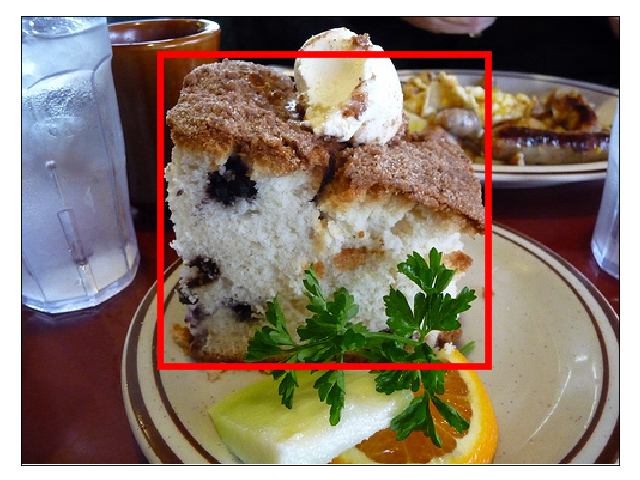
\includegraphics[scale=0.15]{figures/2390077_1254219_supercat_unique.png} &
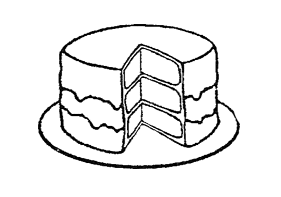
\includegraphics[scale=0.4]{figures/snodgrass_vanderwart_cake_042.png}\\
 cake\ (53),  food\ (19), bread\ (8), burger\ (6), dessert\ (6), snacks\ (3), muffin\ (3),  pastry\ (3) & \hspace{.9cm} cake (83)
\end{tabular}
\caption{Names for a cake object in ManyNames (left) and in Snodgrass's Naming Norms (right), percentages of responses in parentheses.}
\label{fig:cake}
\end{figure}



Therefore, we contribute a new dataset, ManyNames, that contains 36 crowd-sourced names for 25K instances from \vg. Thus, the number of annotations per object available in ManyNames is considerably larger than in recent data collections in L\&V and can be used to compute agreement and related measures reliably.
Moreover, our images show objects in complex visual contexts,
unlike the ``clean'' ImageNet data~\cite{imagenet_cvpr09} which is popular in Computer Vision \cite{ILSVRC15}, and unlike stylized line drawings used in picture naming experiments in Cognitive Science (see Figure \ref{fig:cake}).
%

As illustrated for an object of the class ``cake'' in Figure \ref{fig:cake}, our data reveals clear naming preferences (53\% of the annotators prefer the basic-level \textit{cake}) and also rich variation (the remaining annotators prefer other options like \textit{food, dessert, bread}) which is not restricted to taxonomical relations studied in previous work on naming \cite{Ordonez:2016,graf2016animal}.

%%% Local Variables:
%%% mode: latex
%%% TeX-master: "lrec2020naming"
%%% End:
